\subsection*{Recurrent Neural Networks}
Memorize previous output or hidden layer to feed it back in the network in the next iteration.
\setlength{\intextsep}{-5pt}
\begin{wrapfigure}{l}{0.05\textwidth}
    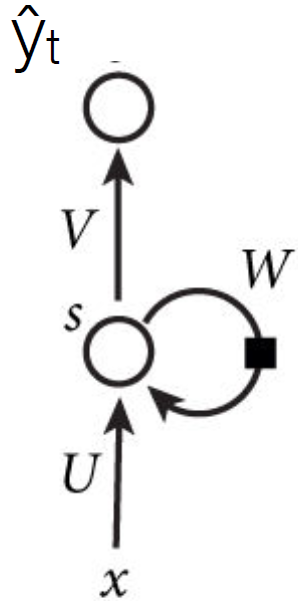
\includegraphics[width=\linewidth]{images/BPTT.png}
\end{wrapfigure}
We sum errors across a sequence of correct outputs $y_t$ and predicted ones
$\hat{y}_t$, treating the sequence as one training example.
$s_t=\text{tanh}(Ux_t+Ws_{t-1})$\\
$\hat{y}_t=\text{softmax}(Vs_t)$\\
$E(y,\hat{y})=-\sum_{t}y_t\log\hat{y}_t$\\
$\frac{\partial E}{\partial W}=\sum_{t}\frac{\partial E_t}{\partial W}$
thus, in general, the larger the temporal horizon, the longer the chain rule of derivatives.
Gradients from distant steps become zero, hindering learning of long-range dependencies.
Modern RNNs use LSTM (Long Short-Term Memory) cells to mitigate this problem.
LSTM cells have a memory cell $c_t$ and three gates: input $i_t$, forget $f_t$ and output $o_t$.